\documentclass[12pt, twoside]{article}
\usepackage[letterpaper, margin=1in, headsep=0.5in]{geometry}
\usepackage[english]{babel}
\usepackage[utf8]{inputenc}
\usepackage{amsmath}
\usepackage{amsfonts}
\usepackage{amssymb}
\usepackage{tikz}
%\usetikzlibrary{quotes, angles}

\usepackage{graphicx}
\usepackage{enumitem}
\usepackage{multicol}

\usepackage{fancyhdr}
\pagestyle{fancy}
\fancyhf{}
\renewcommand{\headrulewidth}{0pt} % disable the underline of the header

\fancyhead[LE]{\thepage}
\fancyhead[RO]{\thepage \\ Name: \hspace{4cm} \,\\}
\fancyhead[LO]{BECA / Dr. Huson / Geometry\\* Unit 6: Distance \& slope\\* 10 January 2019}

\begin{document}
\subsubsection*{7.7b Exam: Similarity ratios, dilation, the tangent function, transformations, symmetry}
  \begin{enumerate}

\item Given the following two linear equations:
  \begin{multicols}{2}
    $l_1: y =\frac{5}{4}x-3$ \\
    $l_2: 5x+4y=8$
  \end{multicols}     \vspace{1cm}
  Write down the slopes of the two lines.
  \begin{multicols}{2}
    $m_1=$ \\
    $m_2=$
  \end{multicols}     \vspace{0.1cm}
  Are the lines parallel, perpendicular, or neither? Justify your answer using the slopes.
  \vspace{2cm}

\item Given $\triangle ABC \sim \triangle DEF$. $m\angle A = 80^\circ$ and $m\angle F = 40^\circ$. Find the measure of $\angle C$. \vspace{2cm}
  
\item In the diagram below of $\triangle ABC$, $D$ is a point on $\overline{BA}$, $E$ is a point on $\overline{BC}$, and $\overline{DE}$ is drawn. \\*[2pt] 
  If $BD=7$, $BA=21$, and $BE=8$, what is the length of $\overline{BC}$ so that $\overline{AC} \parallel \overline{DE}$?
  \begin{flushright}
      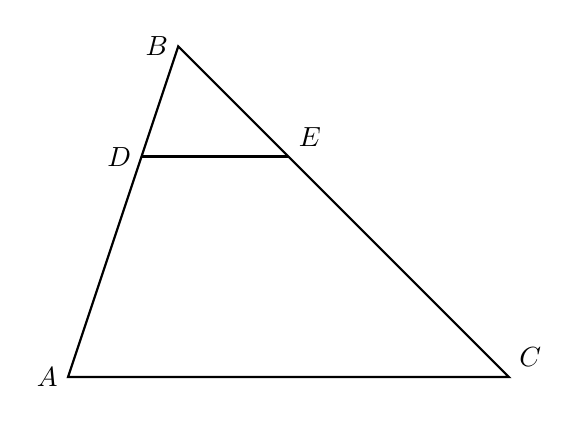
\begin{tikzpicture}[scale=0.7]
        \draw [thick]
        (0,0)node[left]{$A$}--
        (8,0)node[above right]{$C$}--
        (2,6)node[left]{$B$}--cycle;
        \draw [thick]
        (4/3,4)node[left]{$D$}--
        (4,4)node[above right]{$E$};
      \end{tikzpicture}
    \end{flushright}

\item Find the image of $P(3,-5)$ after the translation $(x,y) \rightarrow (x-5,y+8)$.
  
\newpage
\item Graph and label $\triangle ABC$ with $A(0,0)$, $B(5,6)$, and $C(5,0)$. Calculate each length:
  \begin{enumerate}[itemsep=1.4cm]
      \begin{multicols}{2}
      \item $AC=$
      \item $BC=$
      \item $AB=$ \vspace{3cm}
      \begin{center}
        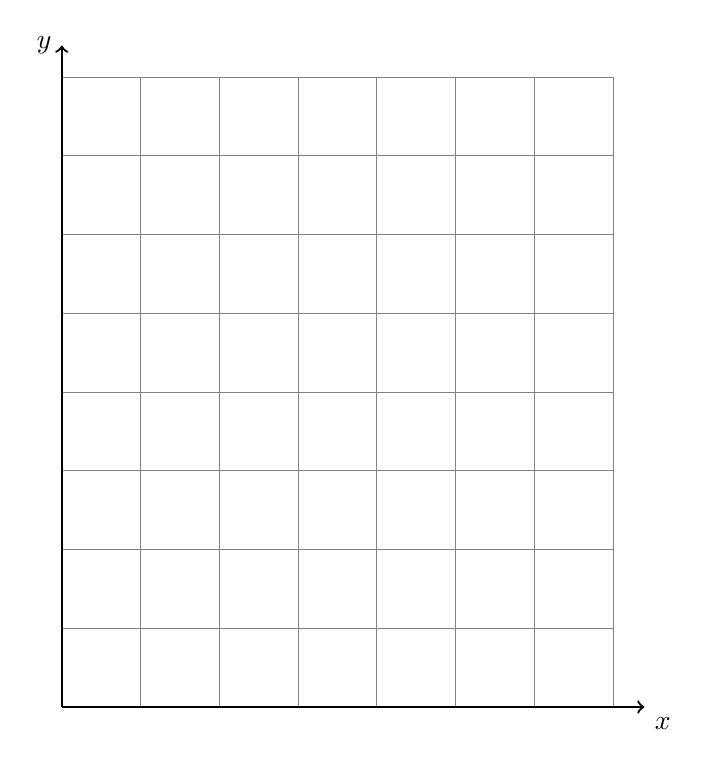
\begin{tikzpicture}
          \draw [help lines] (0,0) grid (7,8);
          \draw [thick, ->] (0,0) -- (7.4,0) node [below right] {$x$};
          \draw [thick, ->] (0,0)--(0,8.4) node [left] {$y$};
        \end{tikzpicture}
      \end{center}
      \end{multicols}%\vspace{2cm}
    \item Write down the equation of the line $\overleftrightarrow{BC}$.
    \item Write down the equation of the line $\overleftrightarrow{AB}$. 
    \item The tangent of an angle is the ratio of the side lengths \emph{opposite} over \emph{adjacent} to the angle. Write down the value as a fraction. \\[0.5cm]
      $\tan \angle BAC=$
    \item Find $m\angle A$ with a calculator's inverse tangent function, $\displaystyle m \angle BAC = \tan^{-1}(\frac{opp}{adj})$, rounded to the \emph{nearest whole degree}.
    \vspace{2cm}
  \end{enumerate}

\newpage
\item Given $\triangle ABP \sim \triangle JKP$ as shown below. $AB=13.5$, $AP=10.0$, $BP=9$, and $JP=27.0$. Find $JK$.
  \begin{flushright}
  \begin{tikzpicture}[scale=1.4]
      \draw [thick]
        (-0.25,-1)node[below left]{$B$}--
        (0.5,2)node[left]{$K$}--
        (4,0)node[below left]{$J$}--
        (0,0)node[above left]{$P$}--
        (-2,0)node[left]{$A$}--cycle;
    \end{tikzpicture}
    \end{flushright}
    \vspace{0.5cm}
    
\item The line $l$ has the equation $y=\frac{3}{2}x+5$. To each line below, circle whether $l$ is parallel, perpendicular, or neither.
  \begin{enumerate}
    \item parallel \quad perpendicular \quad neither \qquad $y=\frac{3}{2}x-2$
    \vspace{0.5cm}
    \item parallel \quad perpendicular \quad neither \qquad $y=\frac{2}{3}x+7$
    \vspace{0.5cm}
    \item parallel \quad perpendicular \quad neither \qquad $3x-2y=-6$
    \vspace{2cm}
  \end{enumerate}

\item $A(-1,4)$ is one endpoint of $\overline{AB}$. The segment's midpoint is $M(3,1)$, as shown below. Find the coordinates of the other endpoint, $B$.
    \begin{flushright}
      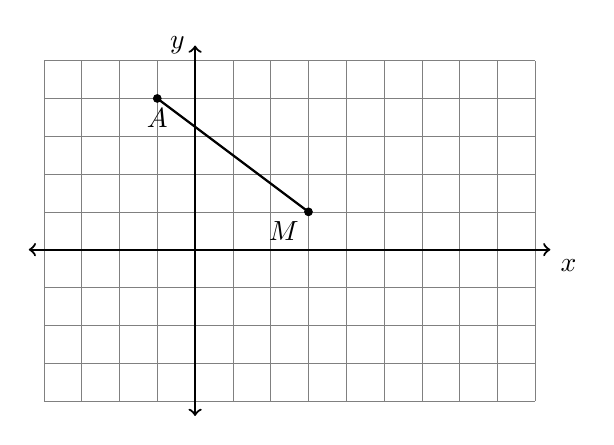
\begin{tikzpicture}[scale=.48]
        \draw [help lines] (-4,-4) grid (9,5);
        \draw [thick, <->] (-4.4,0) -- (9.4,0) node [below right] {$x$};
        \draw [thick, <->] (0,-4.4)--(0,5.4) node [left] {$y$};
        \draw [thick] (-1,4)--(3,1);
        \draw [fill] (-1,4) circle [radius=0.1] node[below] {$A$};
        \draw [fill] (3,1) circle [radius=0.1] node[below left] {$M$};
      \end{tikzpicture}
    \end{flushright}

\newpage
  \item The vertices of $\triangle JKL$ have the coordinates $J(0,0)$, $K(6,0)$, and $L(6,4)$, as shown. \\[0.25cm]
    Apply a dilation to $\triangle JKL \rightarrow \triangle J'K'L'$, centered on the origin and with a scale factor $k=1.5$. Draw the image $\triangle J'K'L'$ on the set of axes below, labeling the vertices, and make a table showing the correspondence of both triangles' coordinate pairs.
      \begin{flushright}
        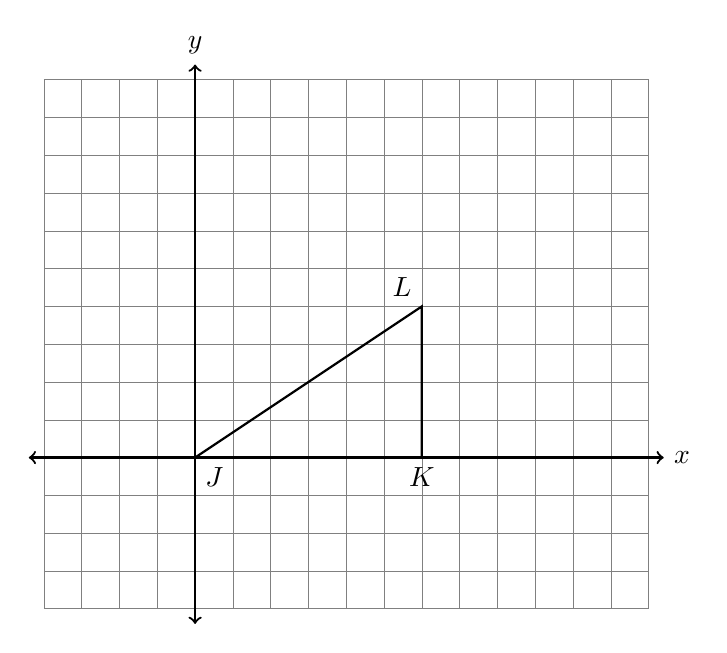
\begin{tikzpicture}[scale=.48]
          \draw [help lines] (-4,-4) grid (12,10);
          \draw [thick, <->] (-4.4,0) -- (12.4,0) node [right] {$x$};
          \draw [thick, <->] (0,-4.4)--(0,10.4) node [above] {$y$};
          \draw [thick]
            (0,0) node[below right] {$J$}--
            (6,0) node[below] {$K$}--
            (6,4) node[above left] {$L$}--
            cycle;
        \end{tikzpicture}
      \end{flushright}

\item Given isosceles $\triangle ABC$ with $\overline{AB} \cong \overline{BC}$, $m\angle A = 53$. Mark and label the diagram, and then find $m\angle B$. \hfill (\emph{the diagram is not to scale})
  \begin{flushright}
  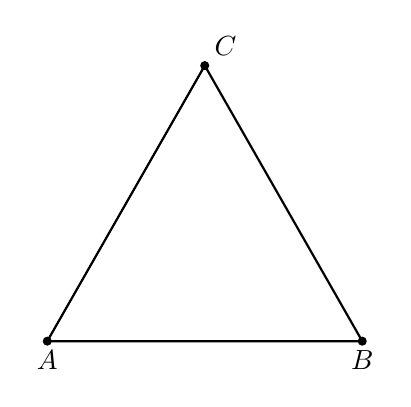
\begin{tikzpicture}[scale=1]
    \draw [thick](0,0)--(4,0)--(2,3.5)--(0,0);
    \draw [fill] (0,0) circle [radius=0.05] node[below]{$A$};
    \draw [fill] (4,0) circle [radius=0.05] node[below]{$B$};
    \draw [fill] (2,3.5) circle [radius=0.05] node[above right]{$C$};
  \end{tikzpicture}
  \end{flushright}

\item A translation maps $N(-3, 7) \rightarrow N'(-4,1)$. What is the image of $M(0,-5)$ under the same translation?

\newpage
\item Solve each equation for $x$, rounding to the nearest hundredth.
  \begin{multicols}{2}
    \begin{enumerate}
    \item $\displaystyle \tan 50^\circ = \frac{x}{10}$ \vspace{5cm}
    \item $\displaystyle \tan 22^\circ = \frac{3}{x}$
    \item $\displaystyle \sin 35^\circ  = \frac{x}{3.5}$ \vspace{5cm}
    \item $\displaystyle \cos 80^\circ = \frac{x}{20}$
    \end{enumerate}
  \end{multicols}
  \vspace{6cm}

\item Solve for $x$, rounding to the nearest whole degree.
  \begin{multicols}{2}
    \begin{enumerate}
    \item $\displaystyle x = \tan^{-1} (\frac{6}{10})$ \vspace{4cm}
    \item $\displaystyle \tan x^\circ = \frac{4.2}{2.9}$ \vspace{4cm}
    \end{enumerate}
  \end{multicols}

\newpage
  \item A dilation centered at $A$ maps $\triangle ABC \rightarrow \triangle ADE$. Given $AB = 9$, $AC = 6$, $BD = 18$, and $DE = 15$. Find  $AD$ and the scale factor $k$. Then find $AE$ and $BC$. %\vspace{1cm}
  \begin{multicols}{2}
    \begin{enumerate}
      \item $AD=$ \vspace{0.3cm}
      \item $k=$ \vspace{0.3cm}
      \item $AE=$ \vspace{0.3cm}
      \item $BC=$
    \end{enumerate}
    \begin{flushright}
      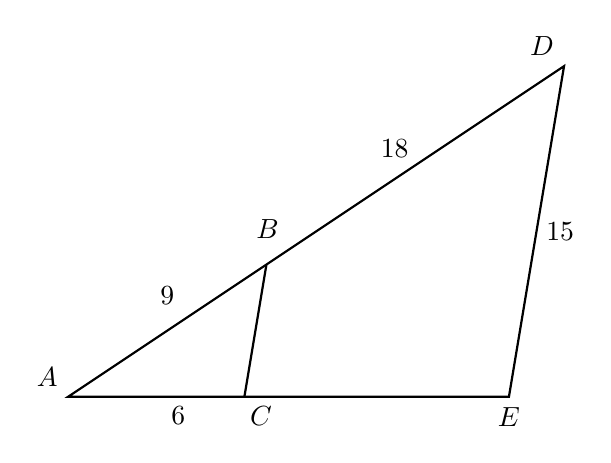
\begin{tikzpicture}[scale=0.7]
        \draw [-, thick] (0,0) node[above left]{$A$}--
        (8,0) node[below]{$E$}--
        (9,6) node[above left]{$D$}--cycle;
        \draw [thick] (3.2,0)--(3.6,2.4);
        \node at (3.5,0) [below]{$C$};
        \node at (4,2.7) [above left]{$B$};
        \node at (2, 0) [below]{$6$};
        \node at (1.8,1.5) [above]{$9$};
        \node at (8.5, 3) [right]{$15$};
        \node at (5.5, 4.5) [right]{$18$}; \vspace{1cm}
      \end{tikzpicture}
    \end{flushright} 
  \end{multicols}\vspace{1cm}

\item The line $\overleftrightarrow{AB}$ has points $A(0,2)$ and $B(4,0)$. Apply a dilation mapping $\overleftrightarrow{AB} \rightarrow \overleftrightarrow{A'B'}$ with a factor of $k=2$ centered at the origin.
  \begin{enumerate}
    \item Draw and label the image on the grid. 
    \begin{flushright} %4 quadrant regents grid w T-Chart
    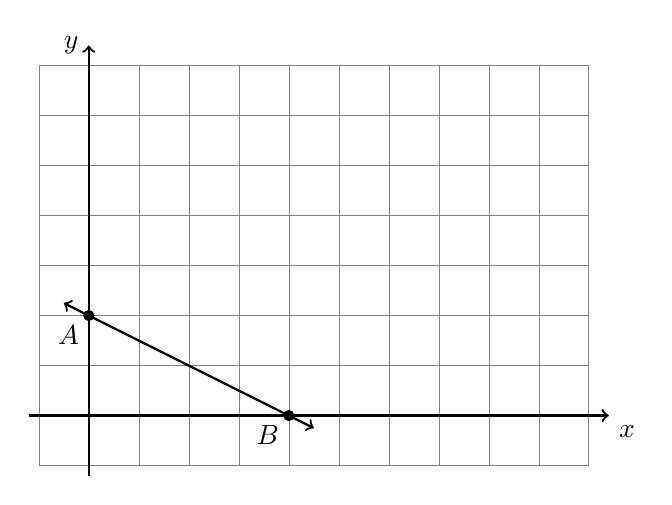
\begin{tikzpicture}[scale=.635]
      \draw [help lines] (-1,-1) grid (10,7);
      \draw [thick, ->] (-1.2,0) -- (10.4,0) node [below right] {$x$};
      \draw [thick, ->] (0,-1.2)--(0,7.4) node [left] {$y$};
      \draw [<->, thick] (-0.5,2.25)--(4.5,-0.25);
      \draw [fill] (0,2) circle [radius=0.1]node[below left]{$A$};
      %\draw [fill] (3,0) circle [radius=0.1]node[below left]{$C$};
      \draw [fill] (4,0) circle [radius=0.1]node[below left]{$B$};
    \end{tikzpicture}
    \end{flushright}
    \item Write the coordinates of the points $A'$ and $B'$.
  \end{enumerate}

\newpage
  \item The side $\overline{AB}$ of triangle $ABC$ is extended and an altitude to the vertex $C$ is drawn, as shown below. The triangle's height is $h=11.0$ and its base measures $AB=19.1$. Find the area of the triangle.
    \begin{flushright}
      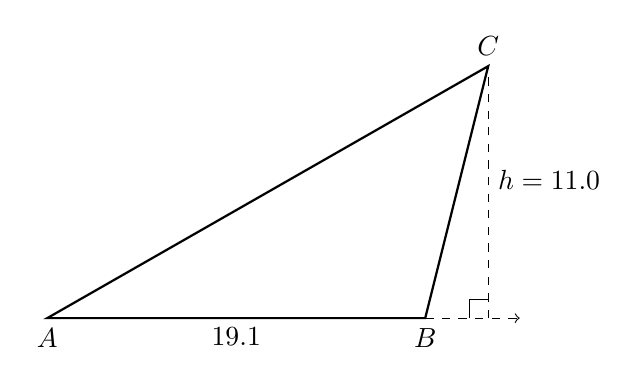
\begin{tikzpicture}[scale=0.8]
        \draw [thick]
          (0,0)node[below]{$A$}--
          (6,0)node[below]{$B$}--
          (7,4)node[above]{$C$} --cycle;
      \draw [dashed] (7,0)--(7,4);
      \draw [dashed, ->] (6,0)--(7.5,0);
      \draw (7,0)++(-0.3,0)--++(0,0.3)--+(0.3,0);
      \node at (7,2.2)[right]{$h=11.0$};
      \node at (3,0)[below]{$19.1$};
      \end{tikzpicture}
    \end{flushright} \vspace{2cm}

  \item Find the midpoint $M$ of $\overline{AB}$ with coordinates $A(-3,1)$ and $B(7, 5)$. Mark and label it on the diagram below.
    \begin{flushright} %4 quadrant regents grid w T-Chart
      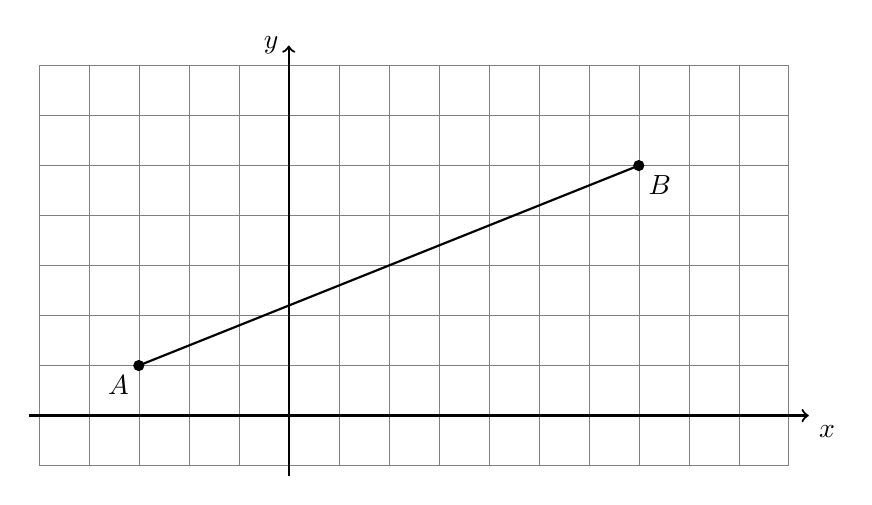
\begin{tikzpicture}[scale=.635]
        \draw [help lines] (-5,-1) grid (10,7);
        \draw [thick, ->] (-5.2,0) -- (10.4,0) node [below right] {$x$};
        \draw [thick, ->] (0,-1.2)--(0,7.4) node [left] {$y$};
        \draw [-, thick] (-3,1)--(7,5);
        \draw [fill] (-3,1) circle [radius=0.1]node[below left]{$A$};
        \draw [fill] (7,5) circle [radius=0.1]node[below right]{$B$};
      \end{tikzpicture}
      \end{flushright}

\newpage
  \item Given two parallel lines and a transversal, as shown below. Given $m\angle 1 = 108^\circ$.
  \begin{center}
  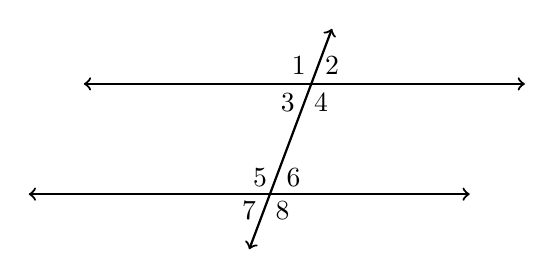
\begin{tikzpicture}[scale=.7]
    \draw [<->, thick] (1,2)--(9,2);
    \draw [<->, thick] (0,0)--(8,0);
    \draw [<->, thick] (4,-1)--(5.5,3);
    \node at (4.5,0.3) [left]{$5$};
    \node at (4.5,0.3) [right]{$6$};
    \node at (4.3,-0.3) [left]{$7$};
    \node at (4.3,-0.3) [right]{$8$};
    \node at (5.2,2) [above left]{$1$};
    \node at (5.2,2) [above right]{$2$};
    \node at (5,2) [below left]{$3$};
    \node at (5,2) [below right]{$4$};
  \end{tikzpicture}
  \end{center}
  \begin{enumerate}
    \item Find the measure $m\angle 2$. \vspace{0.5cm}
    \item Find the measure $m\angle 8$. \vspace{0.5cm}
    \item Given $m\angle 5 = (6x-12)^\circ$. Find $x$. \vspace{4cm}
  \end{enumerate}

\item Given two points $A=-4.7$ and $B=3.3$. Find the value of the midpoint $M$ between $A$ and $B$, and mark and label it on the numberline below.\\[20pt] % Midpoint
    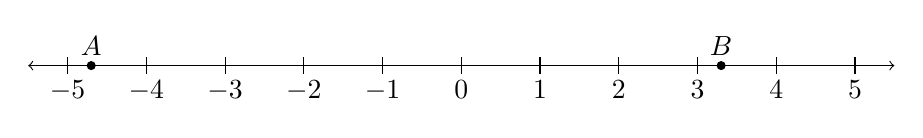
\begin{tikzpicture}
      \draw [<->] (-5.5,0)--(5.5,0);
      \foreach \x in {-5,...,5} %2 leading for diff!=1
        \draw[shift={(\x,0)},color=black] (0pt,-3pt) -- (0pt,3pt) node[below=5pt]  {$\x$};
        \draw [fill] (-4.7,0) circle [radius=0.05] node[above] {$A$};
        \draw [fill] (3.3,0) circle [radius=0.05] node[above] {$B$};
    \end{tikzpicture}

\end{enumerate}
\end{document}